As quarks and gluons have a net colour charge and cannot exist as free particles due to colour-confinement, they can not be observed directly.
After they are produced in the collision, they combine with quarks and anti-quarks spontaneously created from the vacuum
to form a stable configuration of colour-neutral hadrons along the direction of the initial parton.
This happens in a very small timescale, of the order of $10^{-15}$ s, while the involved quarks and gluons are still inside the beam pipe,
and for this reason free quarks and gluons are never observed directly.
The result of this process, called hadronization, is a cone of collimated particles known as a jet.

\subsubsection{Jet Reconstruction}

Jets are the experimental signatures of quarks and gluons produced in high-energy processes such as head-on proton-proton collisions.
They are reconstructed using the anti-$k_t$ clustering algorithm \cite{Cacciari:2008gp}, with a distance parameter of 0.4, on PF candidates.
It defines a distances $d_{ij}$ between the entities i and j, and $d_{iB}$ between object $i$ and the beam (B).:
\begin{equation}
\begin{split}
d_{ij} &= min \left( k^{2p}_{T,i}, k^{2p}_{T,j} \right) \frac{\DR_{ij}}{D^2}\\
d_{iB} &= k^{2p}_{T,i}
\end{split}
\end{equation}
where $k_{T, i}$ is the transverse momentum of the object $i$ and $D$ is the distance parameter that can be adjusted.

The clustering proceeds by identifying the smallest of the distances and if it is a $d_{ij}$ recombining entities i and j,
while if it is $d_{iB}$ calling $i$ a jet and removing it from the list of entities.
The distances are recalculated and the procedure repeated until no entities are left.

In particular, anti-$k_t$ sets $p = -1$, which results in and infrared and collinear safe algorithm, which is resilient to soft radiation,
meaning that soft emissions do not result in irregularities in the boundaries of the resulting jets.

Jets are reconstructed by using the anti-$k_t$ clustering algorithm out of particle flow candidates, with a distance parameter $R = 0.4$,
after rejecting the charged hadrons that are associated to a pileup primary vertex.

\subsubsection{Jet Identification}

In order to assure a good reconstruction efficiency, identification quality criteria are imposed on jets based on
the energy fraction of the charged, electromagnetic, and neutral hadronic components \cite{CMS-PAS-JME-16-003}.

To reduce instrumental background, the tight working point jet ID suggested by the JetMET Physics Object Group is applied.%~\cite{JetID2018}. 
In addition, jets from Pile-Up are rejected using the PileUp jet ID criteria suggested by the JetMET POG.%~\cite{JetPUID2017}.
It is to be noted that the PU JetID was only derived for 2016 conditions but is also applied to 2017 and 2018 samples. 

In this analysis, the jets are required to be within $|\eta| < 4.7$ area and have a transverse momentum above 30 \GeV. 
In addition, the jets are cleaned from any of the tight leptons (passing the SIP and isolation cut computed after FSR correction) 
and FSR photons by a separation criterion: $\Delta R(\text{jet,lepton/photon}) > 0.4$.

In addition this analysis considers also a collection of large radius jets clustered using the same anti-$k_t$ algorithm with a distance parameter $R = 0.8$.
These jets are cleaned using the Pileup Per Particle Identification (PUPPI) \cite{Bertolini_2014}, which is a method for pileup mitigation.

\paragraph{Jet disambiguation\\}
The PF jet collection contains jets clustered with anti-$k_t$ on all the particles reconstructed from Particle Flow.
This means that isolated and energetic leptons and photons, which are part of the signal definition,
are likely to be in the core of a jet due to the nature of the algorithm.
Therefore a disambiguation strategy is needed, to avoid double counting entities.
Jets are removed if they match within $\DR < 0.2$ a photon passing the kinematic selection (Section \todo{ref}),
or a lepton passing the Loose ID.

\subsubsection{Jet Energy Corrections}

The calorimeter response to particles is not linear and it is not straightforward to translate the measured jet energy
to the true particle or parton energy, therefore Jet Energy Corrections (JEC) must be applied.
In this analysis, standard jet energy corrections are applied to the reconstructed jets, which account for pileup,
non uniformity of detector response, and residual differences between the jet energy scale between data and simulation, and residual calibration for data
\cite{CMS:JEC_2011, CMS-DP-2016-020, CMS-DP-2021-033}.
The corrections, parametrized as function of \pt and $\eta$ of the jets, are applied following the standard procedure recommended by CMS jet experts.

\paragraph{Removal of noisy jets\\}
Increased jet multiplicity was reported for 2017 data, creating ``horns'' in the jet $\eta$ distribution for $2.5<|\eta_{jet}|<3$.
The issue was linked to an increase of the ECAL noise, PU and bunch-crossing dependent, thus getting worse as luminosity increases.
The problem can only be fixed in the UL ReReco.
For now, we checked the impact of rejecting jets with raw $\pt < 50 \GeV$ in $2.65 <|\eta| < 3.139$.
As we see no significant impact in the data/MC agreement, we decided not to use these cuts.

\subsubsection{L1 prefiring}

In 2016 and 2017, the gradual timing shift of ECAL was not properly propagated to \Lone trigger primitives (TP)
resulting in a significant fraction of high eta TP being mistakenly associated to the previous bunch crossing~\cite{CMS:L1trigger_Run2}.
Since \Lone trigger rules forbid two consecutive bunch crossings to fire, an unfortunate consequence of this,
in addition to missing the trigger primitive in the correct bunch crossing,
is that events can self veto if a significant amount of ECAL energy is found in the region of $2<|\eta|<3$.
This effect is not described by the simulations.

A similar effect is present in the muon system, where the BX assignment of the muon candidates can be wrong due to the limited time resolution of the muon detectors.
This effect was most pronounced in 2016, but is non-zero for both 2017 and 2018.
The associated prefiring rate is stable for $\pt > 25 \GeV$ but affects the almost entire eta range.
Its magnitude varies between 0\% and a 3\%.

The probability not to prefire (see Equation~\ref{eq:L1prefiring} is calculated for each event and applied as a weight to simulation for 2016 and 2017 samples,
using a software tool developed by CMS \Lone trigger experts.
\begin{equation}
\label{eq:L1prefiring}
w^{pref} = 1 - \Probability(prefire) = \prod_{i\, \in\, \PGg,\, jets,\, \PGm} (1 - \epsilon_i^{pref}(\eta, \pt))
\end{equation}

The Figure~\ref{fig:L1Prefiring} shows the impact of the L1 pre-firing weights on the signal MC.
The impact on the normalization of the signal is around 0.8\%.

\begin{figure}
\subfigure [L1 pre-firing weights]       {\resizebox{.5\textwidth}{!}{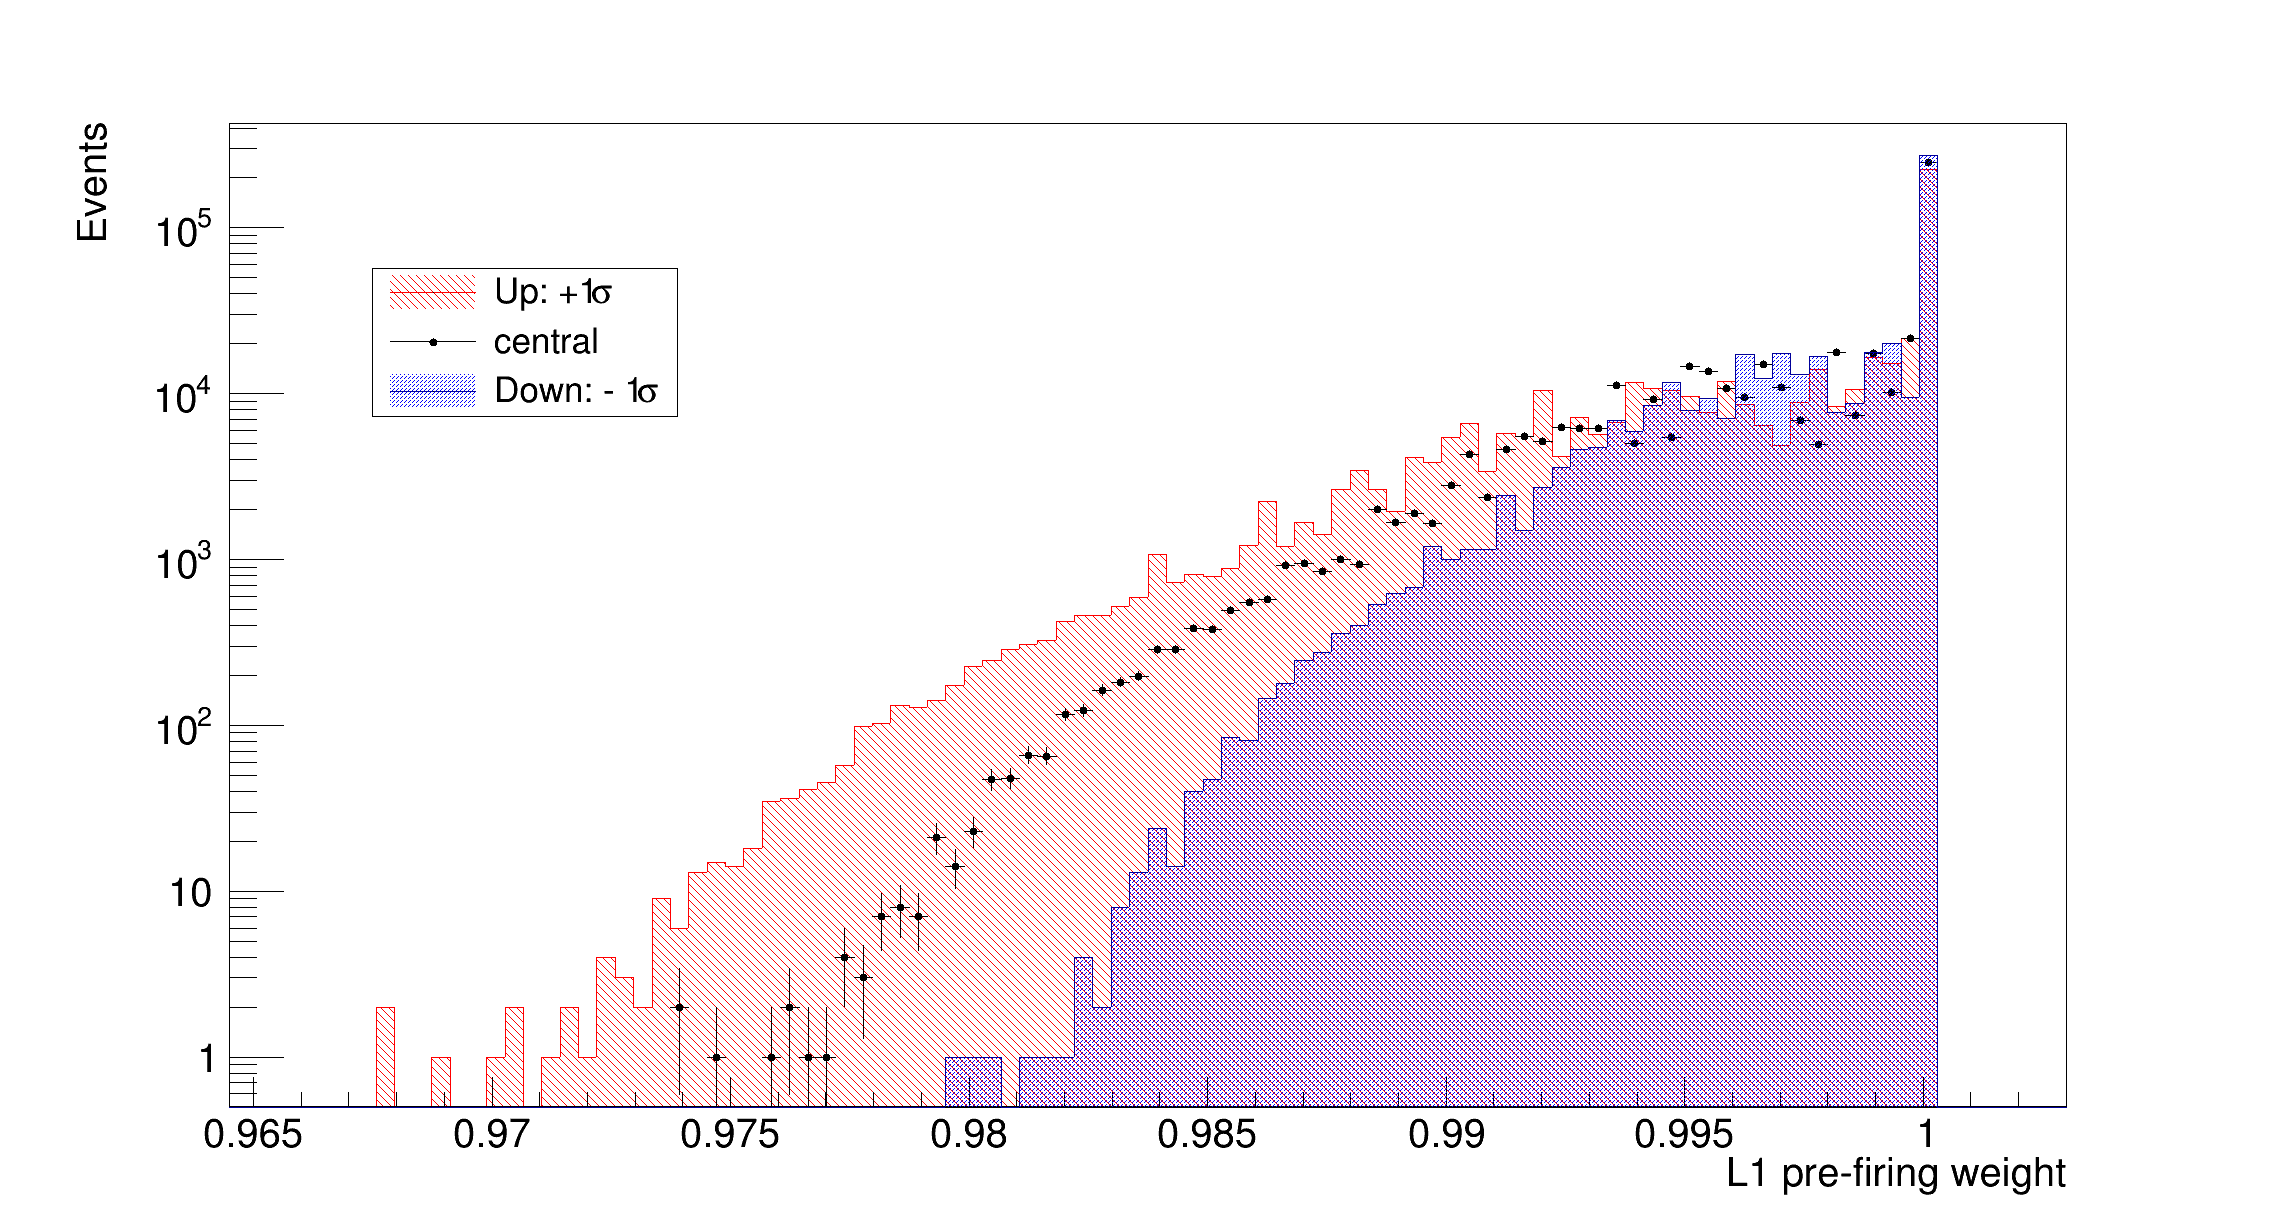
\includegraphics[width=.5\textwidth]{Figures/L1Prefiring_ZZGTo4LG.png}}}
\subfigure [Effect on $m_{4\ell\gamma}$] {\resizebox{.5\textwidth}{!}{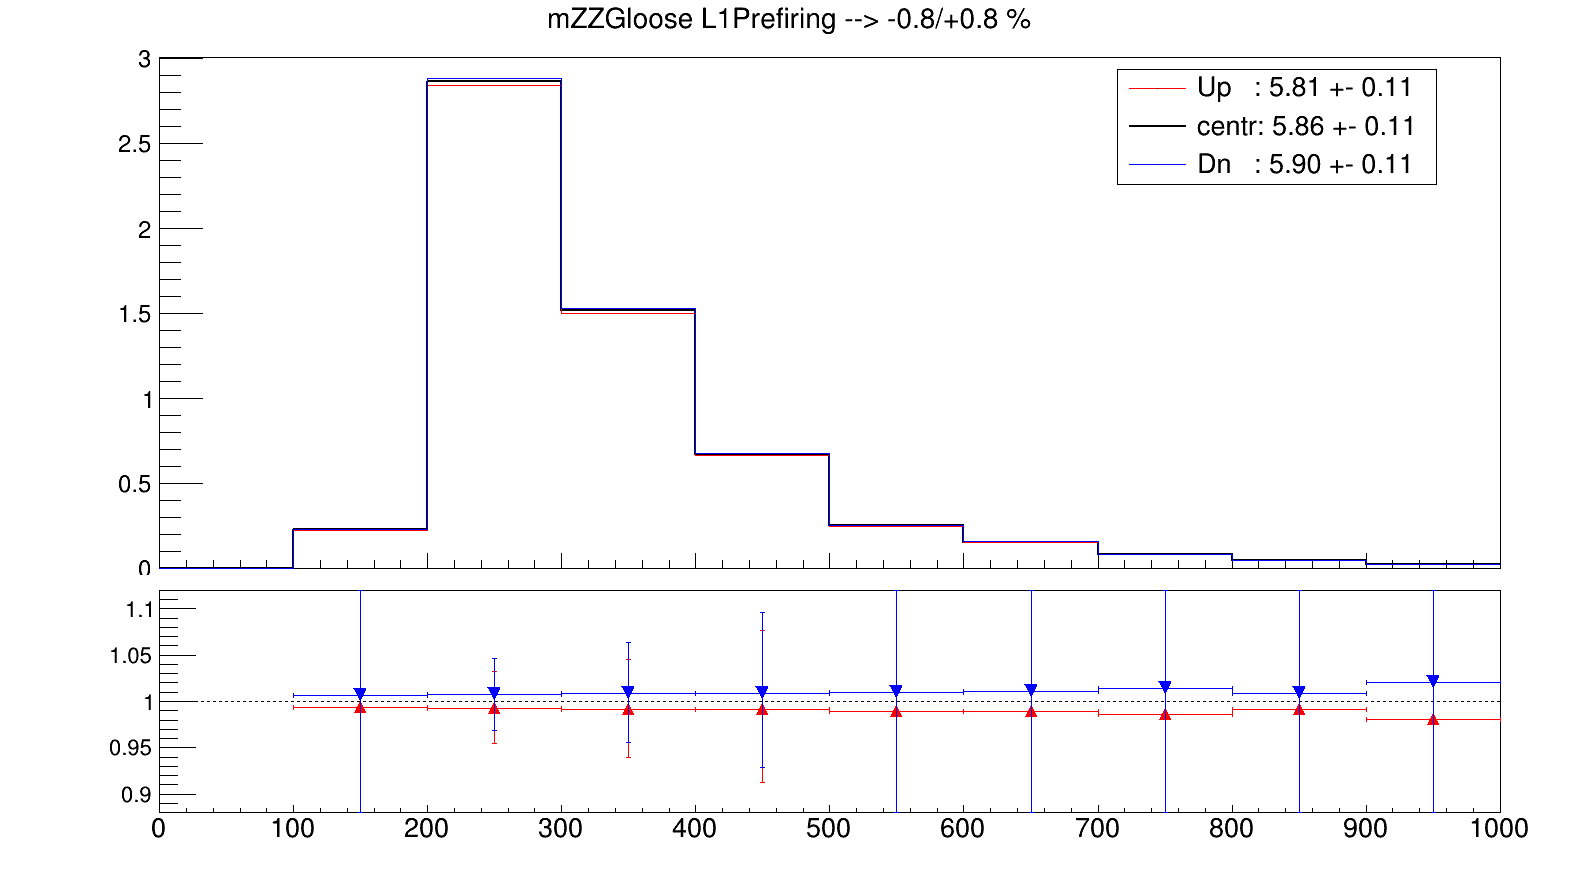
\includegraphics[width=.5\textwidth]{Figures/SYS/SR4P/ZZGTo4LG_mZZGloose_L1Prefiring.png}}}
\caption{L1 pre-firing weights and effect of their application on the signal MC in the signal region with four tight leptons and one photon in 2018.
The photon is required to pass the Loose working point of the cut-based ID.}
\label{fig:L1Prefiring}
\end{figure}
